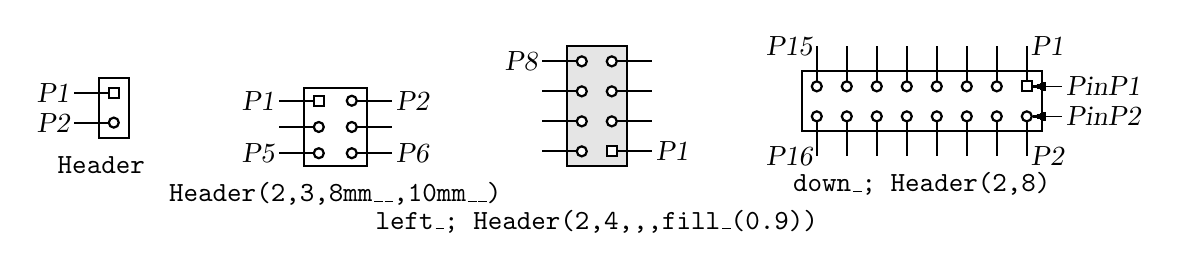
\begin{tikzpicture}[scale=2.54]
% dpic version 2020.03.01 option -g for TikZ and PGF 1.01
\ifx\dpiclw\undefined\newdimen\dpiclw\fi
\global\def\dpicdraw{\draw[line width=\dpiclw]}
\global\def\dpicstop{;}
\dpiclw=0.8bp
\dpiclw=0.8bp
\dpicdraw (0.275,0)
 --(0.275,0.15)
 --(0.125,0.15)
 --(0.125,-0.15)
 --(0.275,-0.15)
 --(0.275,0)\dpicstop
\dpicdraw (0.2,0.075)
 --(0,0.075)\dpicstop
\fill[fill=white,line width=0bp](0.225,0.075)
 --(0.225,0.1)
 --(0.175,0.1)
 --(0.175,0.05)
 --(0.225,0.05)
 --(0.225,0.075)--cycle
\dpicstop
\dpicdraw (0.225,0.075)
 --(0.225,0.1)
 --(0.175,0.1)
 --(0.175,0.05)
 --(0.225,0.05)
 --(0.225,0.075)\dpicstop
\dpicdraw (0.2,-0.075)
 --(0,-0.075)\dpicstop
\dpicdraw[fill=white](0.2,-0.075) circle (0.009843in)\dpicstop
\draw (0,0.075) node[left=-2bp]{\sl P1};
\draw (0.1375,-0.28837) node{\tt Header};
\draw (0,-0.075) node[left=-2bp]{\sl P2};
\dpicdraw (1.464961,-0.09685)
 --(1.464961,0.1)
 --(1.15,0.1)
 --(1.15,-0.293701)
 --(1.464961,-0.293701)
 --(1.464961,-0.09685)\dpicstop
\dpicdraw (1.225,0.034383)
 --(1.025,0.034383)\dpicstop
\fill[fill=white,line width=0bp](1.25,0.034383)
 --(1.25,0.059383)
 --(1.2,0.059383)
 --(1.2,0.009383)
 --(1.25,0.009383)
 --(1.25,0.034383)--cycle
\dpicstop
\dpicdraw (1.25,0.034383)
 --(1.25,0.059383)
 --(1.2,0.059383)
 --(1.2,0.009383)
 --(1.25,0.009383)
 --(1.25,0.034383)\dpicstop
\dpicdraw (1.389961,0.034383)
 --(1.589961,0.034383)\dpicstop
\dpicdraw[fill=white](1.389961,0.034383) circle (0.009843in)\dpicstop
\dpicdraw (1.225,-0.09685)
 --(1.025,-0.09685)\dpicstop
\dpicdraw[fill=white](1.225,-0.09685) circle (0.009843in)\dpicstop
\dpicdraw (1.389961,-0.09685)
 --(1.589961,-0.09685)\dpicstop
\dpicdraw[fill=white](1.389961,-0.09685) circle (0.009843in)\dpicstop
\dpicdraw (1.225,-0.228084)
 --(1.025,-0.228084)\dpicstop
\dpicdraw[fill=white](1.225,-0.228084) circle (0.009843in)\dpicstop
\dpicdraw (1.389961,-0.228084)
 --(1.589961,-0.228084)\dpicstop
\dpicdraw[fill=white](1.389961,-0.228084) circle (0.009843in)\dpicstop
\draw (1.025,0.034383) node[left=-2bp]{\sl P1};
\draw (1.30748,-0.432071) node{\tt Header(2,3,8mm\_\_,10mm\_\_)};
\draw (1.589961,0.034383) node[right=-2bp]{\sl P2};
\draw (1.025,-0.228084) node[left=-2bp]{\sl P5};
\draw (1.589961,-0.228084) node[right=-2bp]{\sl P6};
\fill[fill=white!90!black,line width=0bp](2.464961,0.006299)
 --(2.464961,-0.293701)
 --(2.764961,-0.293701)
 --(2.764961,0.306299)
 --(2.464961,0.306299)
 --(2.464961,0.006299)--cycle
\dpicstop
\dpicdraw (2.464961,0.006299)
 --(2.464961,-0.293701)
 --(2.764961,-0.293701)
 --(2.764961,0.306299)
 --(2.464961,0.306299)
 --(2.464961,0.006299)\dpicstop
\dpicdraw (2.689961,-0.218701)
 --(2.889961,-0.218701)\dpicstop
\fill[fill=white,line width=0bp](2.664961,-0.218701)
 --(2.664961,-0.243701)
 --(2.714961,-0.243701)
 --(2.714961,-0.193701)
 --(2.664961,-0.193701)
 --(2.664961,-0.218701)--cycle
\dpicstop
\dpicdraw (2.664961,-0.218701)
 --(2.664961,-0.243701)
 --(2.714961,-0.243701)
 --(2.714961,-0.193701)
 --(2.664961,-0.193701)
 --(2.664961,-0.218701)\dpicstop
\dpicdraw (2.539961,-0.218701)
 --(2.339961,-0.218701)\dpicstop
\dpicdraw[fill=white](2.539961,-0.218701) circle (0.009843in)\dpicstop
\dpicdraw (2.689961,-0.068701)
 --(2.889961,-0.068701)\dpicstop
\dpicdraw[fill=white](2.689961,-0.068701) circle (0.009843in)\dpicstop
\dpicdraw (2.539961,-0.068701)
 --(2.339961,-0.068701)\dpicstop
\dpicdraw[fill=white](2.539961,-0.068701) circle (0.009843in)\dpicstop
\dpicdraw (2.689961,0.081299)
 --(2.889961,0.081299)\dpicstop
\dpicdraw[fill=white](2.689961,0.081299) circle (0.009843in)\dpicstop
\dpicdraw (2.539961,0.081299)
 --(2.339961,0.081299)\dpicstop
\dpicdraw[fill=white](2.539961,0.081299) circle (0.009843in)\dpicstop
\dpicdraw (2.689961,0.231299)
 --(2.889961,0.231299)\dpicstop
\dpicdraw[fill=white](2.689961,0.231299) circle (0.009843in)\dpicstop
\dpicdraw (2.539961,0.231299)
 --(2.339961,0.231299)\dpicstop
\dpicdraw[fill=white](2.539961,0.231299) circle (0.009843in)\dpicstop
\draw (2.889961,-0.218701) node[right=-2bp]{\sl P1};
\draw (2.614961,-0.570441) node{\tt left\_; Header(2,4,{,},fill\_(0.9))};
\draw (2.339961,0.231299) node[left=-2bp]{\sl P8};
\dpicdraw (4.239961,-0.118701)
 --(4.839961,-0.118701)
 --(4.839961,0.181299)
 --(3.639961,0.181299)
 --(3.639961,-0.118701)
 --(4.239961,-0.118701)\dpicstop
\dpicdraw (4.764961,0.106299)
 --(4.764961,0.306299)\dpicstop
\fill[fill=white,line width=0bp](4.764961,0.081299)
 --(4.789961,0.081299)
 --(4.789961,0.131299)
 --(4.739961,0.131299)
 --(4.739961,0.081299)
 --(4.764961,0.081299)--cycle
\dpicstop
\dpicdraw (4.764961,0.081299)
 --(4.789961,0.081299)
 --(4.789961,0.131299)
 --(4.739961,0.131299)
 --(4.739961,0.081299)
 --(4.764961,0.081299)\dpicstop
\dpicdraw (4.764961,-0.043701)
 --(4.764961,-0.243701)\dpicstop
\dpicdraw[fill=white](4.764961,-0.043701) circle (0.009843in)\dpicstop
\dpicdraw (4.614961,0.106299)
 --(4.614961,0.306299)\dpicstop
\dpicdraw[fill=white](4.614961,0.106299) circle (0.009843in)\dpicstop
\dpicdraw (4.614961,-0.043701)
 --(4.614961,-0.243701)\dpicstop
\dpicdraw[fill=white](4.614961,-0.043701) circle (0.009843in)\dpicstop
\dpicdraw (4.464961,0.106299)
 --(4.464961,0.306299)\dpicstop
\dpicdraw[fill=white](4.464961,0.106299) circle (0.009843in)\dpicstop
\dpicdraw (4.464961,-0.043701)
 --(4.464961,-0.243701)\dpicstop
\dpicdraw[fill=white](4.464961,-0.043701) circle (0.009843in)\dpicstop
\dpicdraw (4.314961,0.106299)
 --(4.314961,0.306299)\dpicstop
\dpicdraw[fill=white](4.314961,0.106299) circle (0.009843in)\dpicstop
\dpicdraw (4.314961,-0.043701)
 --(4.314961,-0.243701)\dpicstop
\dpicdraw[fill=white](4.314961,-0.043701) circle (0.009843in)\dpicstop
\dpicdraw (4.164961,0.106299)
 --(4.164961,0.306299)\dpicstop
\dpicdraw[fill=white](4.164961,0.106299) circle (0.009843in)\dpicstop
\dpicdraw (4.164961,-0.043701)
 --(4.164961,-0.243701)\dpicstop
\dpicdraw[fill=white](4.164961,-0.043701) circle (0.009843in)\dpicstop
\dpicdraw (4.014961,0.106299)
 --(4.014961,0.306299)\dpicstop
\dpicdraw[fill=white](4.014961,0.106299) circle (0.009843in)\dpicstop
\dpicdraw (4.014961,-0.043701)
 --(4.014961,-0.243701)\dpicstop
\dpicdraw[fill=white](4.014961,-0.043701) circle (0.009843in)\dpicstop
\dpicdraw (3.864961,0.106299)
 --(3.864961,0.306299)\dpicstop
\dpicdraw[fill=white](3.864961,0.106299) circle (0.009843in)\dpicstop
\dpicdraw (3.864961,-0.043701)
 --(3.864961,-0.243701)\dpicstop
\dpicdraw[fill=white](3.864961,-0.043701) circle (0.009843in)\dpicstop
\dpicdraw (3.714961,0.106299)
 --(3.714961,0.306299)\dpicstop
\dpicdraw[fill=white](3.714961,0.106299) circle (0.009843in)\dpicstop
\dpicdraw (3.714961,-0.043701)
 --(3.714961,-0.243701)\dpicstop
\dpicdraw[fill=white](3.714961,-0.043701) circle (0.009843in)\dpicstop
\draw (4.764961,0.306299) node[right=-2bp]{\sl P1};
\draw (4.764961,-0.243701) node[right=-2bp]{\sl P2};
\draw (4.239961,-0.382071) node{\tt down\_; Header(2,8)};
\draw (3.714961,0.306299) node[left=-2bp]{\sl P15};
\draw (3.714961,-0.243701) node[left=-2bp]{\sl P16};
\dpiclw=0.4bp
\filldraw[line width=0bp](4.856627,0.126299)
 --(4.789961,0.106299)
 --(4.856627,0.086299) --cycle\dpicstop
\dpicdraw (4.809295,0.106299)
 --(4.939961,0.106299)\dpicstop
\draw (4.939961,0.106299) node[right=-2bp]{\sl PinP1};
\filldraw[line width=0bp](4.856627,-0.023701)
 --(4.789961,-0.043701)
 --(4.856627,-0.063701) --cycle\dpicstop
\dpicdraw (4.809295,-0.043701)
 --(4.939961,-0.043701)\dpicstop
\draw (4.939961,-0.043701) node[right=-2bp]{\sl PinP2};
\dpiclw=0.8bp
\end{tikzpicture}
\vspace*{-0.5\baselineskip}
